\documentclass{scaffold/sigchi}
\usepackage{pifont} % Check marks
\newcommand{\cmark}{\ding{51}} % So we can use \cmark instead of \ding{51}
\newcommand{\xmark}{\ding{55}}
%\usepackage[none]{hyphenat}
\usepackage{makecell} % For table headers
\usepackage{multirow}

% \usepackage[style=numeric,sorting=nty, eprint=false,doi=true,isbn=false,url=false, maxbibnames=99, giveninits=false]{biblatex}
% \DeclareFieldFormat{labelnumberwidth}{#1\adddot\midsentence}

% \addbibresource{sample.bib}

% Title
\def\plaintitle{Impact of Audio and Visual Display of Positive Reinforcement on Supporting Habit Formation}
%\def\plaintitle{Investigating the Impact of Displaying Positive Reinforcement Using Different Modalities on Habit Formation}

% Authors as plain text
\def\plainauthor{First Author, Second Author, Third Author,
  Fourth Author, Fifth Author, Sixth Author}
\def\emptyauthor{}
\def\plainkeywords{habit formation; behaviour change; positive reinforcement}
\def\plaingeneralterms{Documentation, Standardization}
  \usepackage{pgfplots}
  \pgfplotsset{compat=1.12}

% Use this section to set the ACM copyright statement (e.g. for
% preprints).  Consult the conference website for the camera-ready
% copyright statement.

% Copyright
\CopyrightYear{2017}
%\setcopyright{acmcopyright}
\setcopyright{acmlicensed}
%\setcopyright{rightsretained}
%\setcopyright{usgov}
%\setcopyright{usgovmixed}
%\setcopyright{cagov}
%\setcopyright{cagovmixed}
% DOI
\doi{http://dx.doi.org/10.475/123_4}
% ISBN
\isbn{123-4567-24-567/08/06}
%Conference
\conferenceinfo{CHI'18,}{April 21--26, 2018, Montreal, Canada}
%Price
% \acmPrice{\$15.00}

% Use this command to override the default ACM copyright statement
% (e.g. for preprints).  Consult the conference website for the
% camera-ready copyright statement.

%% HOW TO OVERRIDE THE DEFAULT COPYRIGHT STRIP --
%% Please note you need to make sure the copy for your specific
%% license is used here!
% \toappear{
% Permission to make digital or hard copies of all or part of this work
% for personal or classroom use is granted without fee provided that
% copies are not made or distributed for profit or commercial advantage
% and that copies bear this notice and the full citation on the first
% page. Copyrights for components of this work owned by others than ACM
% must be honored. Abstracting with credit is permitted. To copy
% otherwise, or republish, to post on servers or to redistribute to
% lists, requires prior specific permission and/or a fee. Request
% permissions from \href{mailto:Permissions@acm.org}{Permissions@acm.org}. \\
% \emph{CHI '16},  May 07--12, 2016, San Jose, CA, USA \\
% ACM xxx-x-xxxx-xxxx-x/xx/xx\ldots \$15.00 \\
% DOI: \url{http://dx.doi.org/xx.xxxx/xxxxxxx.xxxxxxx}
% }

% Arabic page numbers for submission.  Remove this line to eliminate
% page numbers for the camera ready copy
% \pagenumbering{arabic}

% Load basic packages
\usepackage{balance}       % to better equalize the last page
\usepackage{graphics}      % for EPS, load graphicx instead 
\usepackage[T1]{fontenc}   % for umlauts and other diaeresis
\usepackage{txfonts}
\usepackage{mathptmx}
\usepackage[pdflang={en-US},pdftex]{hyperref}
\usepackage{color}
\usepackage{booktabs}
\usepackage{textcomp}

% Some optional stuff you might like/need.
\usepackage{microtype}        % Improved Tracking and Kerning
% \usepackage[all]{hypcap}    % Fixes bug in hyperref caption linking
\usepackage{ccicons}          % Cite your images correctly!
% \usepackage[utf8]{inputenc} % for a UTF8 editor only

% If you want to use todo notes, marginpars etc. during creation of
% your draft document, you have to enable the "chi_draft" option for
% the document class. To do this, change the very first line to:
% "\documentclass[chi_draft]{sigchi}". You can then place todo notes
% by using the "\todo{...}"  command. Make sure to disable the draft
% option again before submitting your final document.
\usepackage{todonotes}






% llt: Define a global style for URLs, rather that the default one
\makeatletter
\def\url@leostyle{%
  \@ifundefined{selectfont}{
    \def\UrlFont{\sf}
  }{
    \def\UrlFont{\small\bf\ttfamily}
  }}
\makeatother
\urlstyle{leo}




% To make various LaTeX processors do the right thing with page size.
\def\pprw{8.5in}
\def\pprh{11in}
\special{papersize=\pprw,\pprh}
\setlength{\paperwidth}{\pprw}
\setlength{\paperheight}{\pprh}
\setlength{\pdfpagewidth}{\pprw}
\setlength{\pdfpageheight}{\pprh}

% Make sure hyperref comes last of your loaded packages, to give it a
% fighting chance of not being over-written, since its job is to
% redefine many LaTeX commands.
\definecolor{linkColor}{RGB}{6,125,233}
\hypersetup{%
  pdftitle={\plaintitle},
% Use \plainauthor for final version.
%  pdfauthor={\plainauthor},
  pdfauthor={\emptyauthor},
  pdfkeywords={\plainkeywords},
  pdfdisplaydoctitle=true, % For Accessibility
  bookmarksnumbered,
  pdfstartview={FitH},
  colorlinks,
  citecolor=black,
  filecolor=black,
  linkcolor=black,
  urlcolor=linkColor,
  breaklinks=true,
  hypertexnames=false
}

% create a shortcut to typeset table headings
% \newcommand\tabhead[1]{\small\textbf{#1}}

\title{\plaintitle}



\usetikzlibrary{patterns}
% Authors on paper
\numberofauthors{3}
\author{%
  \alignauthor{Leave Authors Anonymous\\
    \affaddr{for Submission}\\
    \affaddr{City, Country}\\
    \email{e-mail address}}\\
  \alignauthor{Leave Authors Anonymous\\
    \affaddr{for Submission}\\
    \affaddr{City, Country}\\
    \email{e-mail address}}\\
  \alignauthor{Leave Authors Anonymous\\
    \affaddr{for Submission}\\
    \affaddr{City, Country}\\
    \email{e-mail address}}\\
}

\begin{document}

\maketitle

\begin{abstract}
Habit formation technologies use rewards and points as means for providing positive reinforcement, often in visual or audio forms such as jingles, badges or animations. Providing the right reward increases the chances for developing a new habit; yet, research on how these rewards should be delivered and the impact that this has on the process of habit formation is scarce. In this paper we investigate how three types of positive reinforcement (audio, visual, audio-visual) influence habit completion and automaticity. We describe a four week study in which participants used a chatbot that delivered different types of rewards for completing a new daily habit. The results reported higher habit completion rates when a reward was present, especially for the audio-visual condition, without necessarily increasing behaviour automaticity. This has implications for the design of habit formation technologies that rely on audio and visual rewards as means of positive reinforcement.
\end{abstract}

\category{H.5.m}{Information interfaces and 
presentation (e.g. HCI)}{Miscellaneous}
\category{H.5.2}{User Interfaces}{User-Centered Design}

\keywords{\plainkeywords}


\section{Introduction}
In recent years, designing technology to support habit formation has become an important theme in HCI research. This is not surprising, as understanding how to design systems that support habit development helps to ensure that they lead to long lasting changes in one's behaviour~\cite{how_to_evaluate_tech_for_behaviour_change}. While there is evidence that that supporting contextual cues, regular repetition and positive reinforcement facilitates the formation of new habits~\cite{article_beyond_self_tracking_designing_apps}, there is little research into the impact of different types of positive reinforcement on habit formation.

Positive reinforcement plays an important role in habit formation. It is used as a reward to reinforce a habit and increase repetition~\cite{positive_reinforcement_pro}. While habit formation technologies use extrinsic rewards to increase task repetition, such as coins and points, studies have shown that extrinsic rewards can reduce motivation and therefore hinder habit development~\cite{article_meta_analytic_review_intrinsic_motivation}. 

%Technology can help people stick to a routine by sending repeated messages and encouraging people~\cite{positive_reinforcement_pro}. However, these techniques do not always work and may build repetitive actions rather than habit automaticity~\cite{coaching_not_that_good}. Therefore, technology should be designed to avoid building repetitive actions and instead build habit automaticity. Repetitive actions lead people to become dependent on technology and when the system is eventually removed, habit performance decreases~\cite{article_dont_kick_habit, article_realtime_feedback_improving_medication_taking}. Habit automaticity is a measure of habit strength~\cite{article_4q_SRBAI} and is the key that removes this dependency~\cite{article_beyond_self_tracking_designing_apps}.

Sending positive text messages to affirm behaviour is one type of positive reinforcement that aims to motivate habit completion~\cite{chi_crowd_designed_motivation}. However, this may simply encourage repetitive actions rather than help to develop automaticity of behaviour that characterises habits~\cite{habits_as_automaticity_not_frequency_gardner}. Coaching a person throughout the habit formation process by guiding them every step of the way encourages habit performance~\cite{coaching_not_that_good}, but can also build dependency when the coach is removed~\cite{article_dont_kick_habit, article_realtime_feedback_improving_medication_taking}. A successful method of positive reinforcement is to build habit automaticity, rather than repetitive actions~\cite{article_beyond_self_tracking_designing_apps}, which can be helped by using intrinsic motivation after a habit is completed~\cite{article_a_self_efficacy, article_meta_analytic_review_intrinsic_motivation}.

When delivered through technology, positive reinforcement aimed at facilitating intrinsic motivation is usually presented in a form of visual feedback~\cite{comparison_of_auditory_visual_feedback, visual_mode_better, article_realtime_feedback_improving_medication_taking}, however only as a means to increase task performance; research investigating the use of other modes for habit formation is scarce. Although auditory feedback has been shown to improve task performance~(e.g.~\cite{burke2006comparing, vazquez2012auditory, chi_oussama_tap_the_shapetones}), it is not known how it affects habit formation.

% The type of intrinsic reward for habit formation has had little research improves motivation to complete a habit, even when the reward is removed~\cite{article_meta_analytic_review_intrinsic_motivation}.

% Motivation can be encouraged by giving people positive reinforcement rewards after they complete an action~\cite{positive_reinforcement_pro}. However, how the reward is delivered and the type of reward used is also crucial to success.

%The method of delivery should suit each individual user and a choice of delivery should be available. For example, a survey on feedback systems~\cite{article_user_centred_multimodal_reminders} advised that delivery of interaction should span different modalities to increase retention and better suit the needs of users. Although interaction across modalities is important, this research does not have configurable feedback, but aims to compare how each type of feedback can affect motivation. Monetary (extrinsic) rewards can hinder motivation~\cite{article_meta_analytic_review_intrinsic_motivation}, whereas, satisfaction-based (intrinsic) rewards can be beneficial to motivation and should be preferred. 
%This study uses a chatbot to deliver intrinsic positive reinforcement rewards from different modalities to see how participants habit automaticity and performance are affected.

To address this gap, we describe a four week situated study that explored the impact of different types of positive reinforcement (audio, visual, audio-visual) on the process of habit formation and motivating repeated behaviour. The main contribution of our work is a better understanding of the effectiveness of these types of positive feedback. We show that visual positive reinforcement can increase habit completion rates, over audio-visual and audio. However, it does not necessarily support habit formation as even though we observed an increase in habit automaticity, the use of specific rewards did not seem to impact this measurement. This has implications for the design of habit formation technologies that rely on audio and visual rewards as means of positive reinforcement.

\section{Background}
\subsection{Role of positive reinforcement in habit formation}
Changing behaviour permanently requires forming a new habit~\cite{article_experiences_of_habit_formation}. The process of creating a new habit takes constant repetitive use~\cite{article_how_habits_formed_modelling_habit_formation}. The easier the action, the shorter the time before the action turns into a habit, from drinking water (18 days), to going to the gym (254 days). Building the habit around an existing routine helps develop the action into a habit~\cite{habits_event_cues_1}. The existing routine acts as a trigger to motivate the desired action~\cite{habits_event_cues_2}, with the context of the routine as the cue for the trigger. Attaching habits onto existing event-based cues are easier to remember~\cite{article_implementation_intentions_multicue} when compared with time-based habits, mainly due to change in time with change in environment, e.g. the weekend~\cite{coaching_not_that_good}. Event-based cues help connect the contextual information with the action and builds habit automaticity~\cite{article_implementation_intentions}.

Positive reinforcement rewards the person by encouraging them to perform the action again until it forms into a habit and some researchers suggest it is the main part of behaviour change~\cite{article_a_self_efficacy}. This reward increases intrinsic motivation by giving the feeling of satisfaction~\cite{article_promoting_habit_formation} and increases the persons perception of their performance~\cite{positive_reinforcement_pro} especially when the task is interesting~\cite{article_meta_analytic_review_intrinsic_motivation}. When designing behaviour change technology, the delivery of the reward must be carefully considered because it can affect the formation of new habits.

\subsection{Providing positive reinforcement with technology}
\emph{[this should be an overview of how behaviour change / habit formation tech provides positive reinforcement. after you give the overview, then we can look into individual modalities]}

\emph{[somewhere in this section we need a description of my 2015 paper and the guidelines for habit formation apps. since the bot's functionality is based on that, we have to introduce it earlier -- KS]}

A large number of habit forming systems are mobile apps~\cite{survey_on_current_apps_of_steel}. But although most of these apps are rated highly, they do not ground themselves in behaviour change theory~\cite{article_beyond_self_tracking_designing_apps, article_dont_kick_habit}. Several studies of these apps suggest that habit performance is not sustained after the app is removed~\cite{survey_on_apps_2,article_dont_kick_habit,article_realtime_feedback_improving_medication_taking}, due to the lack of habit automaticity developed during the habit tracking process. This can be a problem when using mobile apps to consistently manage behaviour and can create a notable difference in the persons behaviour after it is removed~\cite{article_my_phone_is_part_of_my_soul}. Building habit automaticity is the key for removing this dependency but requires the desired action to be built around an existing routine~\cite{article_how_habits_formed_modelling_habit_formation, article_implementation_intentions_multicue}. Technology should help with routine creation by having additional checks to guard against changes in routine that check in with people about their habit if their situation changes~\cite{article_dont_forget_your_pill}. This is vital for sustaining habit completion and building habit automaticity.


Although the majority of these systems are apps~\cite{survey_on_current_apps_of_steel}, there are plenty of other options available when designing behaviour change interventions. One option that has been recently used are \textit{chatbots}. They have been integrated into messaging apps, such as the \textit{Telegram} app to track food habits~\cite{telegram_bot_tracking_habits} and are seen as a significant component of HCI's increasing shift towards new interaction paradigms involving natural language user interfaces% the next big thing in HCI
~\cite{chatbots_and_new_world_of_hci}.


Positive reinforcement feedback can be delivered by technology from different modalities. Audio, visual and audio-visual modes are the most common for issuing feedback in HCI~\cite{desinging_interface_speech_tech}. Feedback from each of these different modalities has been shown to improve task performance for small tasks~\cite{chi_oussama_tap_the_shapetones}. Combining modalities can be useful for issuing user feedback, enabling systems to be accessible to varying ages~\cite{article_user_centred_multimodal_reminders}. Individual modes can improve the effectiveness of reminders~\cite{multi_modal_reminders_less_disruptive, article_designing_multimodal_reminders_for_home}. However, the effectiveness of each type of modality as reward feedback and how combined modalities impact interaction when used by technology has little research. Therefore, technology to support behaviour change should explore a range of modalities for feedback. Research into audio, visual and audio-visual feedback was identified to understand how they impact behaviour and habit formation.

Audio feedback has been shown to improve task success when used as a notification for a task~\cite{auditory_notifications_increase_delivery_success}, but little work has shown how it impacts the completion of habits. Fast visual feedback has been shown to be preferred over audio when the relative importance of the task is high~\cite{visual_mode_better} and has been shown to improve the consistency of a medication taking habit~\cite{article_realtime_feedback_improving_medication_taking}. However, when the visual feedback is removed habit performance can drop, suggesting a dependency on the technology and the visual feedback. Instead these cues should be constructed around another routine to build habit automaticity and allowing for permanent behaviour change after the system is removed. Although audio and visual feedback has been shown to improve task performance, audio-visual has shown to be the best at increasing task performance, than audio or visual alone~\cite{benefits_of_audio_visual_1, benefits_of_audio_visual_2, chi_oussama_tap_the_shapetones}. For example, a meta-analysis of 43 multi-modal studies~\cite{comparing_modalities_effects_of_visual_auditory} revealed it was the most effective at increasing performance when a single task is being performed and when compared with visual or audio feedback alone. However, care needs to be taken when adding an extra modality as this study showed that visual feedback improved task performance, but sacrificed task quality~\cite{comparing_modalities_effects_of_visual_auditory}.

These three types of feedback increase task completion in different ways. However, how this feedback impacts habit formation is unsure. An in-the-wild study to gain insight into audio, visual and audio-visual positive reinforcement impacts habit formation is conducted and detailed below.

\begin{figure}
  \centering
  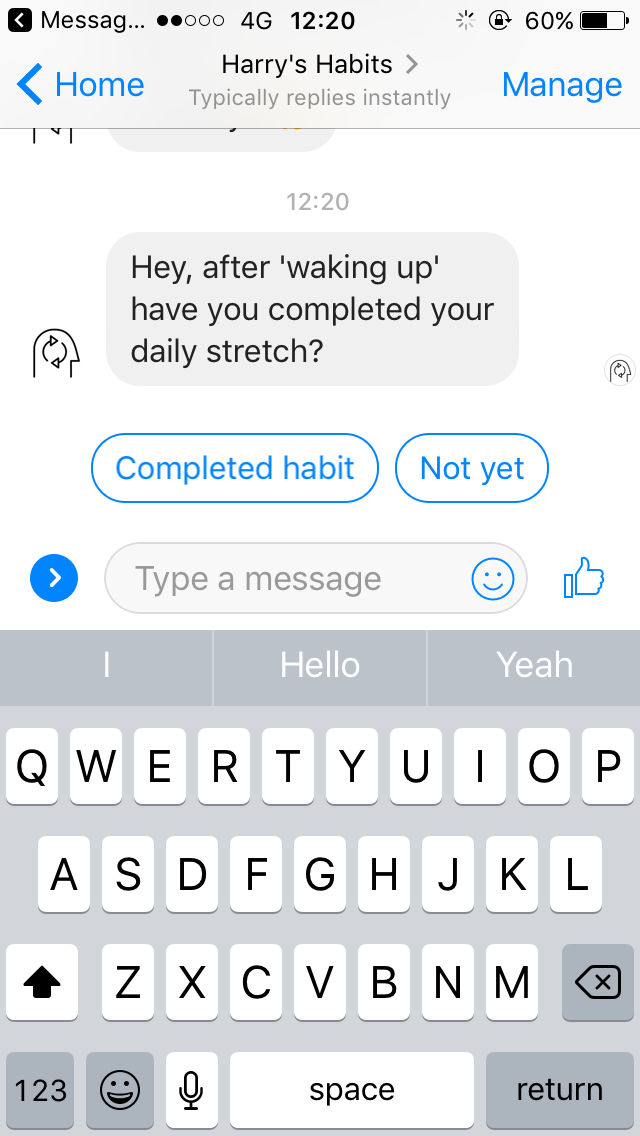
\includegraphics[width=0.47\columnwidth]{figures/reminder.png}
  \hspace{5px}
  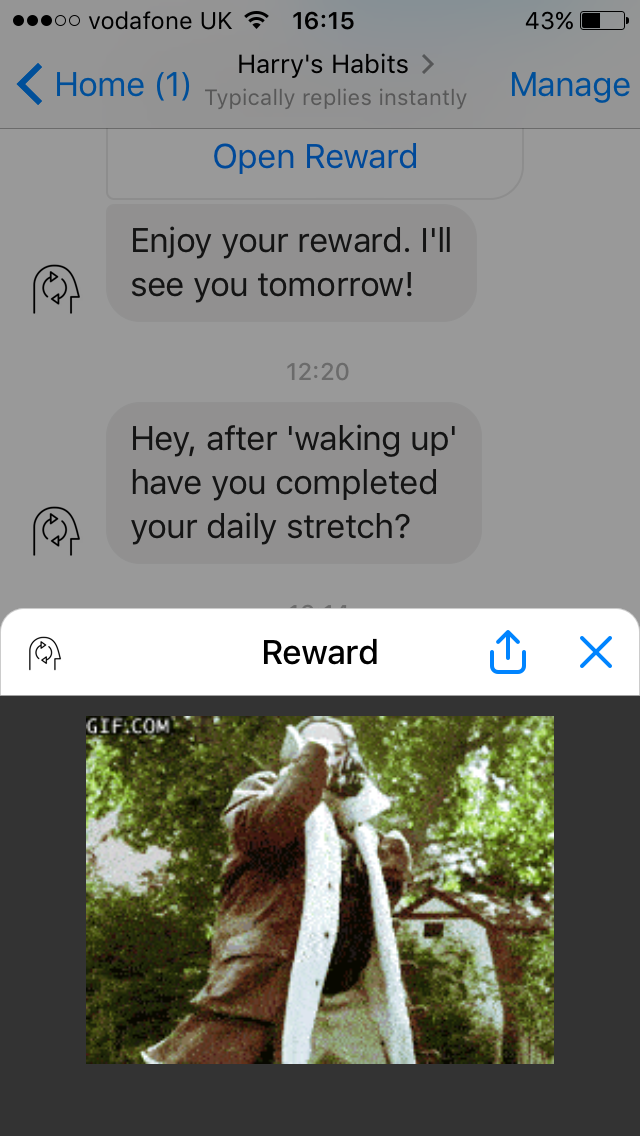
\includegraphics[width=0.47\columnwidth]{figures/reward-visual.png}
  \caption{Bot's ``check in'' message (left) and an example of a reward (right).}~\label{fig:setup}
\end{figure}

\section{Comparing Types of Positive Reinforcement}
The aim of the study was to explore what type of positive reinforcement would be the most effective in supporting regular habit completion and the development of automaticity. We conducted a four week situated study followed by semi-structured interviews to evaluate each reward from a different mode using a chatbot to deliver each reward. The study and the bot are described below.

\subsection{Method}
For the purpose of the study, we developed a chatbot that was used to deliver positive reinforcement to participants wanting to start a new healthy habit. To ensure they were motivated to pursue their habit, we gave them a choice: they could select a physical activity habit (stretching, press ups, the plank) or a relaxing habit (reading, writing, meditation). We selected these specific habits, as they are easy to complete and generally do not require any special equipment. Moreover, simple tasks become automatic quicker than complex actions~\cite{article_how_habits_formed_modelling_habit_formation} and such simple habits allow to observe changes in automaticity of behaviour within four weeks~\cite{article_beyond_self_tracking_designing_apps}. 
The study has been approved by the University Ethics Committee.

\subsubsection{Participants}
Fifty-four participants were recruited on social networks. They were 18-63 years old (mean age=26.7 years old, SD=10), thirty-two, or 59\% were male, fourteen, or 26\% were female, and eight, or 15\%  chose not to disclose their gender; sixteen, or 29\% were university students. As their habit of choice, fifteen participants selected meditation, twelve selected stretching, eleven selected press ups, six selected reading, five selected writing and five selected the plank. In terms of interactions with the bot, twenty-one participants used a web browser, eighteen used iOS devices, twelve used Android and three used other mobile devices to interact with the bot. 

\subsubsection{Design}
Participants were randomly assigned to one of four conditions: Audio, Visual, Audio-Visual and the Control group. Each condition differed by the type of positive reinforcement it provided after participants reported completion of their daily habit: participants in the Audio condition received a fifteen-second audio clip as a reward for completing their habit; in the Visual condition they received a fifteen-second GIF; the Audio-Visual condition combined the audio clip with a GIF; and participants in the Control group received a confirmation message ``Thanks.''. Table 1 summarises study conditions. 

For each condition, we measured the number of times the selected habit was completed during the study. ``Habit completion rate'' was defined as the number of times the person repeated and report the behaviour, divided by twenty-one days during which participants interacted with the bot. We also measured the change in automaticity of the behaviour during the final weeks, to assess habit strength.


\begin{table}[b]
  \centering   
  \begin{tabular}{l l l}
    % \toprule
\multicolumn{1}{l}{\small \textit{Condition}} &
\multicolumn{1}{p{1.4cm}}{\small \textit{Number of Participants}} &
\multicolumn{1}{l}{\small \textit{Positive Reinforcement}} \\
    \midrule
    Audio & 14 & 15s audio\\
    Visual & 15 & 15s GIF \\
    Audio-Visual & 14 & 15s GIF and audio \\
    None (control group) & 11 & Confirmation \\
    % \bottomrule
  \end{tabular}
  \caption{Study conditions and their corresponding types of positive reinforcement.}~\label{fig:precise_rewards}
\end{table}

\subsubsection{Materials}
To deliver different types of positive reinforcement, we built a custom Facebook Messenger bot (see Figure~\ref{fig:setup}). Bot's functionality and approach to support habit formation was informed by~\cite{article_beyond_self_tracking_designing_apps}: rather than providing reminders, the bot first allowed participants to define a routine and during the study provided ``check in'' notifications to see if the routine was followed; if the routine was not working and participants did not complete their habit on time, the bot then suggested changes to the plan. For example, if a participant regularly snoozed the check in notification, the bot would ask the participant if they wanted to move the check in time for later in the day.

We decided to use a bot as it can easily send notifications, is cross-platform and thus highly available, and also offers simple user interface and easy interactions already familiar to the users. Moreover, the integration with the platform meant that interactions with the bot would be visible alongside participant's other conversations, making it easier to report completion of the habit~\cite{the_power_of_logging_mobile_notifications}.

As the aim of the rewards was to motivate the participants to keep coming back every day and completing their habits, we identified several ``motivational'' GIFs and audio files, and each GIF file was tweaked to match the audio frequency. We decided to use popular GIFs with internet memes, i.e. content that is passed along from person to person via social media posts~\cite{meme_definition}. Humorous GIF memes make people laugh and are popular on some social media sites, where they usually are the most engaging content~\cite{meme_gifs_are_good}. Given that our bot was integrated with Facebook, and that Facebook introduced built-in support for animated GIFs~\cite{fb_gif_rollout}, memes would integrate well with the bot environment. 

We also used the bot to collect responses to the Self-Report Behavioural Automaticity Index (SRBAI;~\cite{article_4q_SRBAI}). This is a validated four-item instrument for measuring habit automaticity, which can be used as an indicator of habit strength. %SRBAI statements are presented on a 5-point Likert scale with answers from 'Strongly Disagree' (1) to 'Strongly Agree' (5); higher scores indicate higher self-reported levels of automaticity.

\begin{figure}
  \centering
  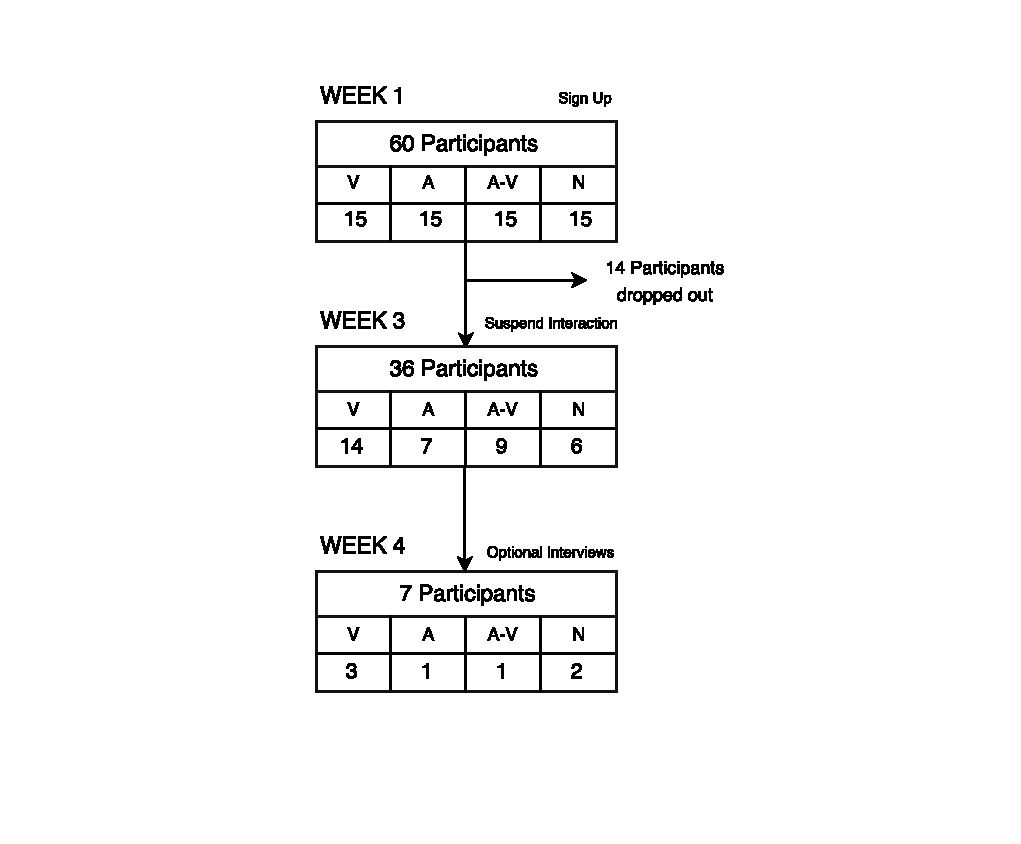
\includegraphics[width=0.7\columnwidth]{figures/study-flow.pdf}
  \caption{Participant drop-out during the four-week study. A: audio, V: visual, A-V: audio-visual, N: no reward.}~\label{fig:study_dropout}
\end{figure}

\subsubsection{Procedure}
Recruitment posts instructed potential participants to connect with our bot via Facebook Messenger. By connecting with the bot, completing the set-up and providing demographics information, participants expressed their consent to participate in the study.

During the set-up process, participants were asked to select one of the healthy habits they would like to develop and, as recommended in~\cite{article_dont_forget_your_pill} for technologies supporting habit formation, to specify contextual cues associated with that habit and the time they would want to complete it (morning, afternoon, evening). Once their habit routine was specified, participants were automatically assigned to one of the study conditions. 

Next, for the first three weeks of the study, participants were asked to complete their chosen habit as part of the specified routine. During that period, the bot ``checked in'' with the participants after their specified time (see Figure~\ref{fig:precise_rewards}, left). Participants then could indicate whether they completed the habit or not. If they reported habit completion, they would receive their positive reinforcement message (see Figure~\ref{fig:precise_rewards}, right). If they selected ``not yet'', the bot would check on the participant again an hour later. This allowed for the checks to be snoozed, to ensure the new habit fits into participant's routine. If participants constantly told the bot they had not completed their habit yet, the bot would suggest making changes to the routine.

Throughout the study, information about how well each participant was performing was not revealed, as streaks can provide motivation~\cite{article_dont_kick_habit}. 

After interacting with the bot for three weeks, participants were asked to complete the SRBAI questionnaire and answer a set of questions about the positive reinforcement they received. Next, during the final week of the study, bot interactions were suspended, but participants were still asked to continue with their habit. At the end of that period, participants were asked to complete the SRBAI questionnaire again along with a few questions about their experience with the reward. 

\subsubsection{Analysis}
The results are grouped into two measurements habit completion and habit automaticity. For each measurement three categories are used for comparison: i) the control group, audio, visual and audio-visual rewards, ii) combined rewards versus the control group, iii) multiple modalities versus singular modes. Participants also had an option to opt-in for an interview to discuss their experience. The interviews were conducted after the four-week study. The interviews explored participants experience with trying to maintain their habit after the interactions with the bot ended, their attitudes towards positive reinforcement and towards the bot itself. The interviews were recorded, transcribed and grouped into three themes: continuation with habit formation, attitudes towards rewards and attitudes towards the chatbot. 

\section{Results}
Thirty-six participants completed the four-week study (see Figure~\ref{fig:study_dropout}); seven of them were from the Audio condition, fourteen from the Visual condition, nine were from Audio-Visual and six from the Control group. They were 18-63 years old (mean=27 years old, SD=12), twenty-three, or 64\% were male, eleven, or 30\% were female and two, or 6\% didn't say. 

Among participants who completed the study, meditation was the most popular habit (twelve participants, or 33\%), followed by press ups (eight participants, or 22\%), then stretching (six participants, or 15\%). Reading and writing were the least common, only selected by four, or 11\% and two, or 5\% respectively.

\subsection{Habit Completion}
% Habit completion Rate= (SUM of habits-completed for condition / 21 (days)) * 100%
% Avg Rate per week = (SUM of habits-completed for condition / <number of people in condition> / 7 (days)) * 100%
Overall, completion rates varied from 5\% to 100\% across individual participants (mean=30\%). The average habit completion rate was the highest for the Audio-Visual condition, with 33\%, followed by 29\% for the Visual condition, 28\% for the control condition and the lowest for Audio, with 14\%. Figure~\ref{fig:habit_completion_1} shows the average completion rate on a weekly basis for all conditions.

\subsubsection{The effect of each condition on habit completion}
To investigate the levels of habit completion per condition, we conducted a one-way ANOVA. The analysis (see Figure~\ref{fig:habit_completion_1}) revealed that there was a statistically significant difference between each reward ($F(2,624) = 27.007$, $p < 0.05$). A Tukey post hoc test revealed that the difference in completed habits was significantly lower for the Audio ($0.081 + 0.274$, $p < 0.005$), Control group ($0.182 + 0.386$, $p < 0.005$) and Audio-Visual ($0.267$ + $0.484$, $p = 0.025$) feedback conditions compared to the Visual feedback ($0.373$ + $0.484$) condition.



\begin{figure}
\centering
 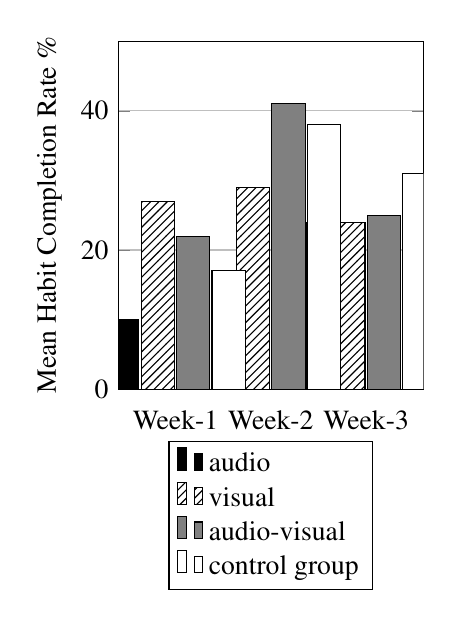
\begin{tikzpicture}
   \begin{axis}[
      width  = 0.45*\textwidth,
      height = 6cm,
      major x tick style = transparent,
      ybar=2*\pgflinewidth,
      bar width=12pt,
      ymajorgrids = true,
      symbolic x coords={Week-1, Week-2, Week-3},
      xtick = data,
      scaled y ticks = false,
      enlarge x limits=0.3,
      ymin=0,
      ymax=50,
      legend cell align=left,
      legend style={at={(0.5,-0.15)},anchor=north},
      ylabel={Mean Habit Completion Rate \%},
   ]
   
      \addplot[style={fill=black},error bars/.cd, y dir=both, y explicit,error bar style=red]
           coordinates { % Audio
          (Week-1, 10)
          (Week-2, 0)
          (Week-3, 24)
           };


      \addplot[style={fill=white},  postaction={
        pattern=north east lines
    }, error bars/.cd, y dir=both, y explicit]
          coordinates { % Visual
          (Week-1, 27)
          (Week-2, 29)
          (Week-3, 24)
      };


      \addplot[style={fill=gray},error bars/.cd, y dir=both, y explicit,error bar style=red]
           coordinates {  % audio-visual
          (Week-1, 22)
          (Week-2, 41)
          (Week-3, 25)
      };
           
      \addplot[style={fill=white},error bars/.cd, y dir=both, y explicit,error bar style=red]
           coordinates { % Control
          (Week-1, 17)
          (Week-2, 38)
          (Week-3, 31)
      };
      \legend{audio, visual, audio-visual, control group}

  \end{axis}
  \end{tikzpicture}
  \caption{The effect of each condition on habit completion.}~\label{fig:habit_completion_1}
\end{figure}



\begin{figure}
  \centering
 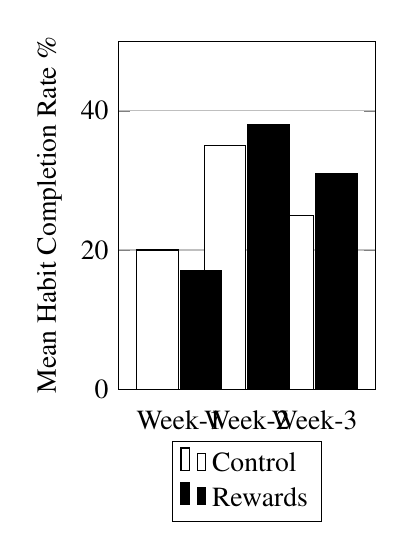
\begin{tikzpicture}
   \begin{axis}[
      width  = 0.4*\textwidth,
      height = 6cm,
      major x tick style = transparent,
      ybar=2*\pgflinewidth,
      bar width=15pt,
      ymajorgrids = true,
      symbolic x coords={Week-1, Week-2, Week-3},
      xtick = data,
      scaled y ticks = false,
      enlarge x limits=0.45,
      ymin=0,
      ymax=50,
      legend cell align=left,
      legend style={at={(0.5,-0.15)},anchor=north},
      ylabel={Mean Habit Completion Rate \%},
   ]
      \addplot[style={fill=white},error bars/.cd, y dir=both, y explicit]
          coordinates { % Rewards
          (Week-1, 20)
          (Week-2, 35)
          (Week-3, 25)
          };

      \addplot[style={fill=black},error bars/.cd, y dir=both, y explicit,error bar style=red]
           coordinates {  % Control group
     	  (Week-1, 17)
          (Week-2, 38)
          (Week-3, 31)
           };

      \legend{Control, Rewards}

  \end{axis}
  \end{tikzpicture}
  \caption{The rewards effect on habit completion.}~\label{fig:habit_completion_2}
\end{figure}

\subsubsection{The rewards effect on habit completion}
To explore the effect of rewards on the number of habits completed, compared with the control group, a one-way between-groups analysis of variance with planned comparisons was conducted. Participants were divided into two groups: group one with rewards, group two without rewards. There was a statistically significant difference at the $p$ $<$ $0.005$ level in both groups for week one and three: week one, $F(1,23.20) = 9.48$, $p = 0.005$, week two, $F(1,33.35) = 4.46$, p = 0.42 and week three, $F(1,50) = 17.01$, $p\leq 0.005$. The effect size for week one, week two and week three are large, calculated using $\eta^{2}$, were 0.25, 0.39 and 0.43 respectively, reporting a large difference in the mean scores.


\subsubsection{Multiple vs. single-mode feedback on habit completion}
The results from our study report a significant increase in habit completion for multiple modes (audio-visual). The significance of this finding was tested by conducting a one-way between-groups ANOVA with planned comparisons (see Figure~\ref{fig:habit_completion_3}). Participants were divided into two groups according to their mode. Group one: audio rewards and visual rewards, group two: audio-visual rewards. There was a statistically significant difference between groups each week ($p$ $<$ $0.005$) week one, $F(1,50) = 0.69$, $p = 0.410$, week two, $F(1,50) = 23.04$, $p$ $<$ $0.005$ and week three, $F(1,50) = 8.85$. The effect size for week one, week two and week three are large, calculated using $\eta^{2}$, were 0.25, 0.39 and 0.43 respectively, reporting an increasing difference in the mean scores throughout weeks.


\begin{figure}
  \centering
 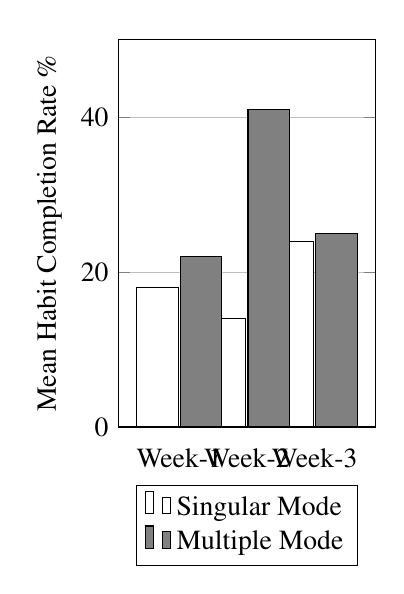
\begin{tikzpicture}
   \begin{axis}[
      width  = 0.4*\textwidth,
      height = 6.5cm,
      major x tick style = transparent,
      ybar=2*\pgflinewidth,
      bar width=15pt,
      ymajorgrids = true,
      symbolic x coords={Week-1, Week-2, Week-3},
      xtick = data,
      scaled y ticks = false,
      enlarge x limits=0.45,
      ymin=0,
      ymax=50,
      legend cell align=left,
      legend style={at={(0.5,-0.15)},anchor=north},
      ylabel={Mean Habit Completion Rate \%},
   ]
      \addplot[style={fill=white},error bars/.cd, y dir=both, y explicit,error bar style=red]
           coordinates { % Singular Modes
          (Week-1, 18)
          (Week-2, 14)
          (Week-3, 24)
      };

      \addplot[style={fill=gray},error bars/.cd, y dir=both, y explicit]
          coordinates { % Multiple Modes
          (Week-1, 22)
          (Week-2, 41)
          (Week-3, 25)
       };

      \legend{Singular Mode, Multiple Mode}

  \end{axis}
  \end{tikzpicture}
  \caption{Multiple vs. single-mode feedback on habit completion.}~\label{fig:habit_completion_3}
\end{figure}

\subsection{Habit Automaticity}
Participants completed SRBAI questionnaires at the end of week three and week four. Eleven participants completed both SRBAI questionnaires: two from the Audio condition, five from Visual, two from Audio-Visual and two from the control group.

\subsubsection{The effect of each condition on habit automaticity}
There was no statistically significant difference between scores as determined by a one-way ANOVA (see Figure~\ref{fig:habit_automaticity_1}) for SRBAI one ($F(3,7) = 0.333$, $p = 0.802$) and SRBAI two ($F(3,7) = 0.639$, $p = 0.614$). For each reward specifically a Tukey post hoc test revealed that there was no significant difference for each reward.
% A paired-samples t-test was conducted on both questionnaires, showing a statistically significant increase in automaticity scores from week three (mean SRABI score = 14.18, SD = 3.78) to week four (mean = 15.09, SD = 4.34), $t(10) = 2.469$, $p$ $<$ $0.005$ (two-tailed). This meant that participant's habit automaticity did generally increase, as reported by a mean increase in SRBAI scores of 0.90 (CI = 95\%, from 0.08 to 1.72) and a large effect size as measured by $\eta^{2} = 0.37$.

\begin{figure}
  \centering
 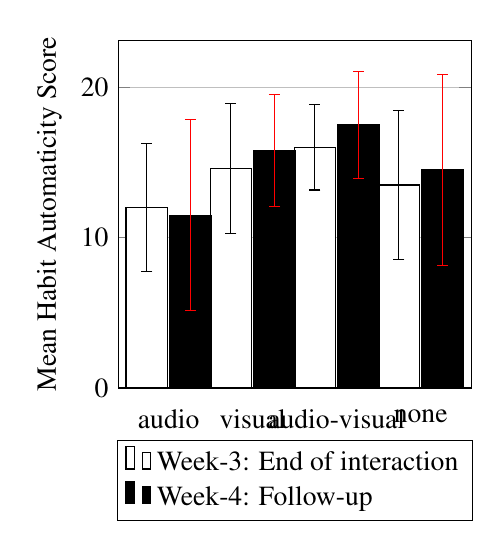
\begin{tikzpicture}
   \begin{axis}[
      width  = 0.5*\textwidth,
      height = 6cm,
      major x tick style = transparent,
      ybar=2*\pgflinewidth,
      bar width=15pt,
      ymajorgrids = true,
      symbolic x coords={audio, visual, audio-visual, none},
      xtick = data,
      scaled y ticks = false,
      enlarge x limits=0.2, % how far apart the bars are, the lower the further apart
      ymin=0,
      legend cell align=left,
      legend style={at={(0.5,-0.15)},anchor=north},
      ylabel={Mean Habit Automaticity Score},
   ]
      \addplot[style={fill=white},error bars/.cd, y dir=both, y explicit]
          coordinates {
          (audio, 12) += (0,4.243) -= (0,4.243)
          (visual, 14.6) += (0,4.336) -= (0,4.336)
          (audio-visual, 16) += (0,2.828) -= (0,2.828)
          (none, 13.5) += (0, 4.950) -= (0, 4.950)
          };

      \addplot[style={fill=black},error bars/.cd, y dir=both, y explicit,error bar style=red]
           coordinates {
          (audio, 11.5) += (0,6.364) -= (0,6.364)
          (visual, 15.8) += (0,3.701) -= (0,3.701)
          (audio-visual, 17.5) += (0,3.536) -= (0,3.536)
          (none, 14.5) += (0, 6.364) -= (0, 6.364)
           };

      \legend{Week-3: End of interaction, Week-4: Follow-up}

  \end{axis}
  \end{tikzpicture}
  \caption{The effect of each condition on habit automaticity.}~\label{fig:habit_automaticity_1}
\end{figure}

\subsubsection{The effect of rewards on habit automaticity}
Comparing participants SRBAI results' with the control group shows the impact rewards had on automaticity.
% An independent-samples t-test was conducted to compare both SRBAI one and SRBAI two for rewards and control (see Figure~\ref{fig:habit_automaticity_2}). For SRBAI one, there was also no significant differences in scores for rewards (mean = 14.33, SD = 3.84) and control (mean = 13.50, SD = 4.94; $t(9) = 0.224$, $p = 0.85$,
% two-tailed). The magnitude of the differences in the means (mean difference = 0.83,
% 95\% CI: \-29.43 to 27.76) was very small ($\eta^{2} = 0.005$). For SRBAI 2, there was no significant difference in scores for rewards
% (mean = 15.22, SD = 4.29) and control (mean = 14.50, SD = 6.36; $t(9) = 0.202$, $p = 0.84$,
% two-tailed). The magnitude of the differences in the means (mean difference = 0.72,
% 95\% CI: \-8.80 to 7.36) was very small ($\eta^{2} = 0.004$). Another test was conducted to validate this finding.
A one-way between-groups ANOVA with planned comparisons was also conducted, but there was not a statistically significant difference for the two groups at SRBAI 1: $F(1,9) = 0.02$, $p = 0.88$, and SRBAI two: $F(1,9) = 0.07$, $p = 0.78$. In addition, the difference in mean scores between the groups had, at SRBAI one: a medium effect with an effect size $\eta^{2} = 0.11$, and at SRBAI two: a large effect, with an effect size of $\eta^{2} = 0.17$.

\begin{figure}
  \centering
 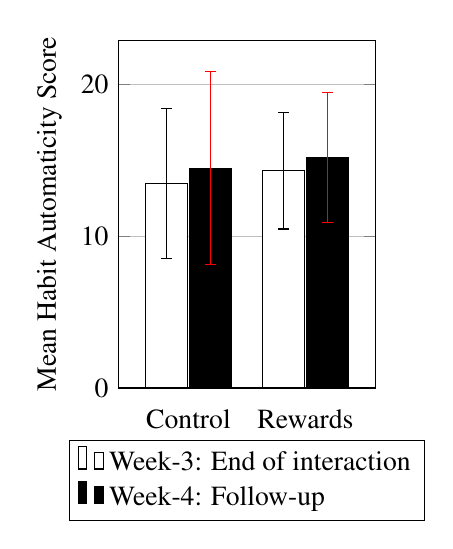
\begin{tikzpicture}
   \begin{axis}[
      width  = 0.4*\textwidth,
      height = 6cm,
      major x tick style = transparent,
      ybar=2*\pgflinewidth,
      bar width=15pt,
      ymajorgrids = true,
      symbolic x coords={Control,Rewards},
      xtick = data,
      scaled y ticks = false,
      enlarge x limits=0.60,
      ymin=0,
      legend cell align=left,
      legend style={at={(0.5,-0.15)},anchor=north},
      ylabel={Mean Habit Automaticity Score},
   ]
      \addplot[style={fill=white},error bars/.cd, y dir=both, y explicit]
          coordinates {
          (Control, 13.5) += (0,4.94) -= (0,4.94)
          (Rewards, 14.33) += (0,3.84) -= (0,3.84)
          };

      \addplot[style={fill=black},error bars/.cd, y dir=both, y explicit,error bar style=red]
           coordinates {
           (Control, 14.5) += (0,6.36) -= (0,6.36)
           (Rewards, 15.22) += (0,4.29) -= (0,4.29)
           };

      \legend{Week-3: End of interaction, Week-4: Follow-up}

  \end{axis}
  \end{tikzpicture}
  \caption{The effect of rewards on habit automaticity.}~\label{fig:habit_automaticity_2}
\end{figure}

\subsubsection{Multiple vs. single-mode feedback on habit automaticity}
To compare the effect audio-visual had on automaticity a one-way between-groups ANOVA with planned comparisons was conducted (see Figure~\ref{fig:habit_automaticity_3}). Participants were divided into two groups according to their reward mode: group one: audio rewards and visual rewards and group two: audio-visual rewards. There was not a
statistically significant difference for the two groups at SRBAI one: $ F(1,9) = 1.04$, $p = 0.33$, and SRBAI two: $F(1,9) = 0.64$, $p = 0.44$. In addition, the difference in mean scores between the groups had, at SRBAI one: a medium effect with an effect size of $\eta^{2} = 0.11$, and at SRBAI two: a large effect, with an effect size of $\eta^{2} = 0.17$.


\begin{figure}
  \centering
 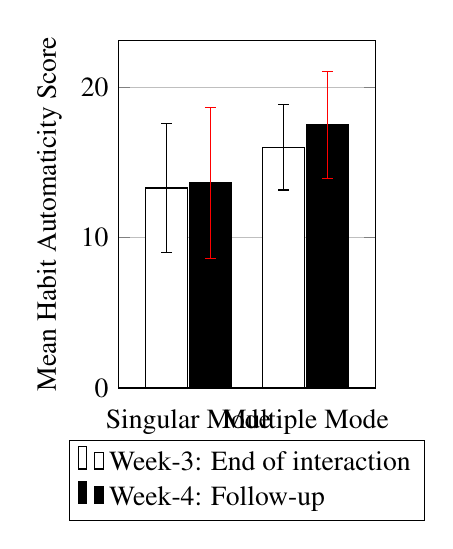
\begin{tikzpicture}
   \begin{axis}[
      width  = 0.4*\textwidth,
      height = 6cm,
      major x tick style = transparent,
      ybar=2*\pgflinewidth,
      bar width=15pt,
      ymajorgrids = true,
      symbolic x coords={Singular Mode, Multiple Mode},
      xtick = data,
      scaled y ticks = false,
      enlarge x limits=0.60,
      ymin=0,
      legend cell align=left,
      legend style={at={(0.5,-0.15)},anchor=north},
      ylabel={Mean Habit Automaticity Score},
   ]
      \addplot[style={fill=white},error bars/.cd, y dir=both, y explicit]
          coordinates {
          (Singular Mode, 13.3) += (0,4.289) -= (0,4.289)
          (Multiple Mode, 16) += (0,2.828) -= (0,2.828)
          };

      \addplot[style={fill=black},error bars/.cd, y dir=both, y explicit,error bar style=red]
           coordinates {
          (Singular Mode, 13.65) += (0,5.033) -= (0,5.033)
          (Multiple Mode, 17.5) += (0,3.536) -= (0,3.536)
           };

      \legend{Week-3: End of interaction, Week-4: Follow-up}

  \end{axis}
  \end{tikzpicture}
  \caption{Multiple vs. single-mode feedback on habit automaticity.}~\label{fig:habit_automaticity_3}
\end{figure}



\subsection{Interview Feedback}
Seven participants agreed to participate in optional interviews. Their details are summarised in Table~\ref{table:transcript_participant_breakdown}. Below we summarise the key findings related to participants' experiences of repeating the habit and support provided by the bot, their attitudes towards types of positive reinforcement they received, and towards the bot itself.

\begin{table}[b]
  \begin{tabular}{l l l l l l}
    \multicolumn{1}{l}{\small \textit{~}} &
    \multicolumn{1}{l}{\small \textit{Age}} & 
    \multicolumn{1}{l}{\small \textit{Gender}} & 
    \multicolumn{1}{l}{\small \textit{Condition}} &
    \multicolumn{1}{l}{\small \textit{Habit}} &
    \multicolumn{1}{p{1cm}}{\small \textit{Completion rate}} \\
    \midrule
    P1 & 24 & M & Visual & Meditation & 86\% \\
    P2 & 19 & F & Auditory & Stretch & 43\% \\ 
    P3 & 28 & F & Visual & Writing & 38\% \\
    P4 & 57 & F & No reward & Meditation & 80\% \\ 
    P5 & 25 & M & Visual & Meditation & 19\% \\ 
    P6 & 21 & F & No reward & Meditation & 33\% \\ 
    P7 & 32 & M & Visual-Auditory & Stretch & 90\% \\
  \end{tabular}
  \caption{Details of participants who were interviewed.}~\label{table:transcript_participant_breakdown}
\end{table}

\subsubsection{Continuation with habit completion}
When discussing the experiences with habit formation, we asked participants for their reasons of selecting their habits. P4 and P5 admitted choosing their habit because they had wanted to start that particular habit for a long time. P2 said that it was \textit{'not too much effort'} and P6 said it was \textit{'something successful people do'}. P7 wanted \textit{'to be more active'} P2 wanted a habit that was \textit{'less time consuming'}. Finally, P1, P5 and P6 wanted to \textit{'relieve stress'}. 

In terms of habit completion, while most participants were able to do it regularly, P6 reported always putting the message off and eventually their habit completion got \textit{'worse and worse'} until they stopped altogether. After the bot was removed, the same was true for all other interviewed participants, who admitted finding it difficult to continue with their habit. They \textit{'kept forgetting'} (P3), found it \textit{'harder to remember'} (P1) and lacked motivation, not performing the action if it had \textit{'been a long day'} (P5). P5 also tried to do it \textit{'every now and again'}, but usually they would only complete it if \textit{'they remembered'}. P1, P4, P6, and P7 all discussed not being able to remember to complete their habit after the bot was removed. This reveals the dependency between technology and habits, suggesting that the bot did not increase habit automaticity, or that the existing routine participants chose was not suitable for new habits, or that they were not given enough time to develop automaticity.

\subsubsection{Attitudes Towards Rewards}
Participants had mixed feelings about the rewards. Some \textit{'did not like the [visual] rewards'} (P1), skipping over them after the first few, they \textit{'just wanted to get rid of the notification dot'} (P1). Another participant (P3) said \textit{'some of them [audio-visual rewards] were funny'}, but they did not like them overall and mentioned the audio rewards were \textit{'too random'}. One participant (P5) thought the rewards did not give them an incentive towards their habit, just a \textit{'nice little extra'} and they discussed including time-sensitive rewards, as they did not want to listen to music before going to bed. This shows the importance of using an appropriate modality at particular times, e.g. not having audio rewards at certain times of the day. Finally, an upbeat participant (P7) talked about \textit{'always wanting to open them'} and \textit{'the combination was perfect'}. However, they said they also found them \textit{'repetitive'} (P7) and one participant stated that they simply wanted to get rid of the notification (P1). This implies that the bot was not tracking how many habits that participant completed, but instead tracking how many times that participant wanted the bot to stop messaging them.

\subsubsection{Attitudes Towards the Chatbot}
Participants were asked about how they found the chatbot as the method of interaction. They found the method \textit{'pretty good'} (P2), they \textit{'liked it'} (P3) and \textit{'would have liked more interaction'} (P4). Suggesting additional features, such as \textit{'help and support throughout'} (P4), \textit{'ideas on how to improve your habit'} (P4) and \textit{'advice on how to set aside time for your habit'} (P4). Others were neutral, some expecting \textit{'different messages, such as Hey [name], a bit more care about the person, a bit less like a robot'} (P7). Four participants (P2, P4, P6, P7) enjoyed the check-in notification aspect, but one found it \textit{'repetitive'} (P7) and \textit{'got annoying if I pressed Not Yet'} (P5). Participants (P1, P3) wanted to see their progress as they tracked their habits, they talked about wanting to reflect on their data. They mentioned that they would feel \textit{'more encouraged to keep doing it, rather than random music [audio rewards]'} (P3). Six out of the seven participants wanted the prototype to come back with a few modifications (P1 was neutral): \textit{'enclosed with Fitbit so it is all in a single place'} (P2), \textit{'fine without rewards'} (P1, P3), \textit{'more interaction'} (P4) and \textit{'with statistics about my progress'} (P1, P3). Participants wanted the bot as more of a \textit{'constant persistent reminder'} (P6) with additional tracking elements to remind them to perform their habit to fit into their busy schedule. Five participants mentioned the \textit{headspace} app (\url{www.headspace.com}), mentioning that they wanted a combination of the bot and headspace. It prompted another participant to download the headspace app. They wanted the bot to keep on track of their habit and they would use the headspace app to help them perform their mindfulness.

Participants gave additional feedback by simply messaging the bot. They asked inquisitive questions, such as \textit{'what kind of thing are you looking to find out'} (P8), \textit{'this is not working for me'} (P9) and \textit{'stop'} (P10)) --- to try and stop the daily messages (the participant then blocked the bot). Negative feedback towards the rewards and bot were also expressed. When asked about being messaged every day, a participant sent this reply and then blocked the bot: \textit{'Do not do that, it will be annoying'} (P11), and another said \textit{'never message me'} (P12). Another stated that this was the \textit{'lame same band'} (P13) after receiving an audio reward.

Participants were able to personalise the chatbot with several different variable configurations. This personalisation could have effected the findings by not narrowing the condition variables. Replicating this research with tighter a configuration is needed to validate this line of reasoning. Finally, streaks could have been better used to give insight to participants progress and challenged them to maintain it, using loss aversion~\cite{loss_aversion} to compare the impact of their broken streak with the gain of keeping it. However, all seven participants interviewed struggled with maintaining habit completion after the bot was removed. This suggests a dependence between the technology and the habit as participants depended on bot notifications to continue repeating the desired action.

\subsection{Summary}
There was a statistically significant drop in habit completion for the control group without rewards. This reveals the effect the rewards had on participant interaction with the bot and habit completion. The findings show that participants are more likely to complete their habit if given one of the rewards, especially if the reward was audio-visual. Although participants enjoyed the rewards at the beginning, most participants disliked them after the first week. However, the results report that participants completed more habits with audio-visual rewards than audio rewards or visual rewards, with audio rewards leading to significantly lower completed habits. Although, participants with audio-visual rewards had higher habit automaticity scores compared with audio or visual rewards, this difference was not statistically significant. Finally, participants picked habits they wanted to perform, but when the bot stopped notifying them, they lacked motivation to completed their habit. Therefore, it is inconclusive whether the rewards or the combined modalities effected habit automaticity. 

\section{Discussion}
What the study was about

What we found out

Did it match the literature? Link back to it

What are the implications for these findings?


Multiple modes as feedback has been shown to increase task completion rates~\cite{comparing_modalities_effects_of_visual_auditory, benefits_of_audio_visual_1, benefits_of_audio_visual_2}. This was mirrored in our results.

This research aimed to understand more about rewards from different modalities and their role in habit formation. Participants receiving bot-delivered rewards completed more habits than the control group without rewards. There was a significant correlation between the habit formation method and habit automaticity. However, this was contradicted during the participant interviews where all seven participants reported a drop in habit completion after one week without the prototype.

There is a significant difference between the audio-visual modes on the number of completed habits. But the result appears to be different to the initial hypotheses, with more participants completing habits with audio rewards and visual rewards than audio-visual. This contradicts existing literature reporting feedback from multiple modes benefits task completion~\cite{}, however these findings are only impacted by the rewards used in this study delivered by the bot. Therefore, it is inconclusive whether audio-visual rewards in a general sense decrease habit completion and visual rewards increase habit completion.

Each individual reward did not have a significant effect on habit automaticity. Although participants with rewards had slightly higher automaticity scores and follow up interviews suggest that automaticity did not develop with participants discussing negative feelings towards rewards during the interviews.  



% \emph{[this section needs cleaning up - leave only bits that are directly linked to the findings and our contribution as outlined in the Introduction. Also, make sure to link the findings and discuss everything in the context of the the literature you described earlier - which of our findings confirm what we know from the literature? which contradict the literature? have we found something completely new and/or unexpected?]}

% Under half the participants completed the modality survey (N = 12, 40\%). These had the following rewards: visual rewards had the highest score (the higher, the more participants preferred the reward) (mean = 12, SD = 3.347), visual and audio rewards were slightly below (mean = 10.75, SD = 1.893).
% TODO: Compare these results to people not using the chatbot, e.g.. people signing up to the gym, new years resolution


% Participants had mixed feelings towards the bot. Their performance shows that the number of snoozes over time decreased, but the number of total habits completed per day also decreased for all reward types (including the control group). However, participant streaks over time increased and 36 participants manage to use it for three weeks.

% Participants had various issues with bot interaction. Seven participants tried to message the bot during setup, instead of using the built in \textit{quick reply} buttons. This broke the setup flow and they had to start again. Other participants tried to send multiple messages when asked for free input, they went around an endless loop when asking for a habit type and participants tried to mark their habit as completed using the Facebook Messenger thumb emotion (which the bot was not coded for). A participant also pointed out that they could change their existing routine time but were unable to change the description.


% The chatbot rewards from different modalities effected habit formation with the singular modes improving habit completion, but not habit automaticity. Feedback towards interaction with the chatbot was mostly positive, but all interviewed participants suggested features they would like, likely because it did not fulfil their needs. The rewards delivered by the chatbot got a mixed reception from participants and did not significantly increase habit automaticity, but they did improve the number of habits participants completed. Therefore, the chatbot is partially effective for supporting habit formation.

% \subsection{Dependence}
% Streaks could have been better used to give insight to participants progress and challenged them to maintain it, using loss aversion~\cite{loss_aversion} to compare the impact of their broken streak with the gain of keeping it. However, all seven participants interviewed struggled with maintaining habit performance after the bot was removed. This suggests a dependence between the technology and the habit as participants depended on bot notifications to continue repeating the desired action.

\subsection{Limitations and Future Work}

This research has a few key limitations that open up future work avenues. First, the small number of participants and the small sample of rewards used in the study make it unclear how these findings would generalise to other types of rewards with the same modality. However, our findings already suggest that...  [explain why it's okay and not a big deal!]


\textbf{Limitations and Future work for Habit Completion:} This research relies on participants self-reporting and participants could have lied to remove the alert instead of performing the habit, just to get the reward. This is particularly true with the snooze function, as the voluntary interviews report that some participants found the bot annoying and stopped using it over time. These participants could have been simply getting rid of the check-in notification rather than completing the habit changing the measurement to how participants reacted to these check-in notifications, instead of their habit. Therefore, it is difficult to draw any valid conclusion on actual habit performance. Future work into how quickly participants responded to the alerts and if the device delivery (browser or smartphone) would better understand how participants interacted with the alerts.



Only seven participants responded to the follow up interviews. In addition, the study relied on participants recall which could be inaccurate. Future work conducting similar research with a larger sample size for the SRBAI questionnaire would validate the effect these rewards had on automaticity.

In addition, future work could focus on comparing bot-delivered positive reinforcement to more traditional approaches, such as SMS or app notifications. With their ease of implementation and access to a large pool of potential participants, chatbots are a promising platform for delivering behaviour change interventions. However, this new method of delivery is another variable and might have affected our results. Therefore, further research into the effect of bot interactions on habit formation is needed to further validate this approach.   

\section{Conclusions}
The results found that the rewards did not impact habit automaticity, but it increased generally, while using the bot. However, the rewards did improve the number of habits people completed, with the highest completion rates for audio-visual rewards. Habit completion was also affected by the different modalities, with audio-visual rewards reporting the highest habit completion when compared with the others. Finally, the limitations of the study do not show any clear statistical significance whether the audio and visual rewards affected habit automaticity. More conclusive evidence is needed to show that rewards from combined modalities effect habit formation. We hope this research opens up new avenues for using bots as tools to help form new habits and give new behaviour change technology insights into positive reinforcement rewards from audio, visual and audio-visual modalities.

% -- FINDINGS --
% AUTOMATICITY
% Bot increased automaticity
% Specific rewards didn't increase automaticity

% COMPLETION
% Visual rewards then audio had highest completion increase
% Audio-Visual rewards actually decreased completion

\section{Acknowledgements}
[Removed for peer review.]
%"Internal reviews" sound a bit like it's been reviewed somewhere, so let's hide it for now.

% Thank you to all the participants involved who provided feedback throughout the study.

\balance{}

% % Either:
% %  1. Put \balance in the first column of the last page
% %  2. Don't use \balance
% %  3. hard-code a column break into the bbl file (before submission)
% % see more http://stackoverflow.com/questions/2149854/how-to-manually-equalize-columns-in-an-ieee-paper-if-using-bibtex
% \balance{}

\bibliographystyle{scaffold/SIGCHI-Reference-Format}
\bibliography{sample}
% \printbibliography

\end{document}
